\chapter{Caracterización del  electroimán} \chapterlabel{Informe/3-CaracterizacionElectroiman} \label{cap:CaracterizacionElectroiman}

\noindent Para el desarrollo del proyecto se dispone \colorbox{red}{cambiar}ya de un electroimán que funcionará como actuador del sistema. A partir de sus características constructivas, y del modelo físico y dinámico del problema, se podrán determinar otros parámetros del sistema de control.

\noindent\colorbox{yellow}{podría ser así...}
\noindent Para el desarrollo del proyecto se utiliza un electroimán disponible en la cátedra que funcionará como actuador del sistema. A partir de sus características constructivas, y del modelo físico y dinámico del problema, se podrán determinar otros parámetros del sistema de control.

\section{Diseño del electroimán} \label{section_disenio_electroimán}



\noindent El electroimán está compuesto por dos piezas: una con forma de “E” y otra con forma de “I”. Estas se construyen a partir del apilado de láminas de acero al silicio de $0.5\:mm$ de espesor, cuyas dimensiones se muestran en la figura \ref{fig:img_plano_dimensiones}. El apilado de las láminas es tal que la rama central de la E tiene una sección cuadrada de $25\:cm^{2}$ lo que maximiza el área mientras que disminuye el perímetro.

\begin{figure}[H]
	\centering
	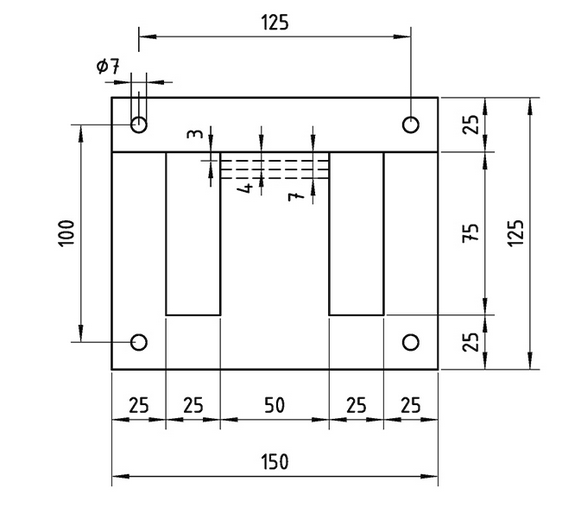
\includegraphics[width=\textwidth]{plano_dimensiones.png}
	\caption{Dimensiones del electroimán}
	\label{fig:img_plano_dimensiones}
\end{figure}

\noindent El bobinado está conformado por $150$ vueltas de alambre de cobre esmaltado de $2.5\:mm$ de diámetro enrollado alrededor de un carrete de plástico (figura \ref{fig:img_carrete}) que luego se ubica en la rama central de la pieza E.

\begin{figure}[H]
	\centering
	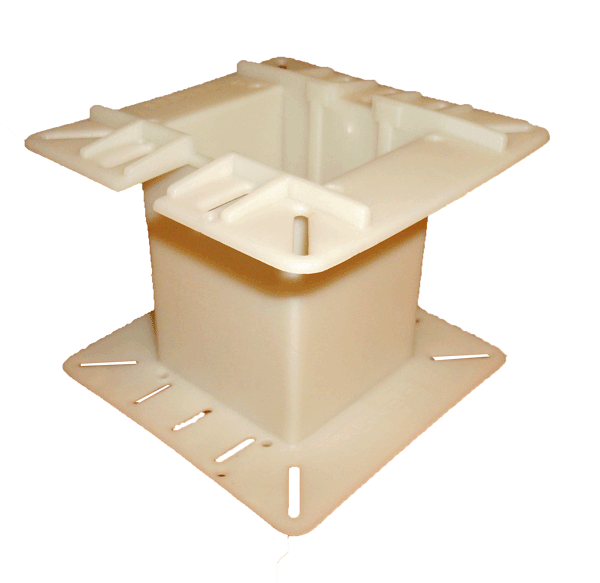
\includegraphics[scale=0.4]{carrete.png}
	\caption{Carrete de plástico para el bobinado}
	\label{fig:img_carrete}
\end{figure}


\noindent Se utiliza un apilado de láminas cuyo exterior está recubierto por una pintura esmaltada para aislarlas entre sí con el fin de minimizar las pérdidas de energía causadas por las corrientes eléctricas que se generan en el núcleo debidas al flujo magnético. 

\noindent Está construido por una laminación normalizada sin desperdicio 600. Estas son útiles ya que cada par de laminas E e I puede fabricarse a partir de una lámina de acero rectangular, de manera de que no se desperdicia material durante la fabricación. 
\colorbox{red}{poner figura del electroimán real????}

\noindent \colorbox{red}{para la foto} El electroimán en el que se basó el diseño del sistema se muestra en la figra
%\noindent Está compuesto por dos piezas: una con forma de “E” y otra con forma de “I”. En su núcleo tiene un bobinado de 150 vueltas (N) de cobre esmaltado con un diámetro de $2.5$ mm. El núcleo es de sección cuadrada ya que esto maximiza el área mientras que disminuye el perímetro, reduciendo así la longitud media de las espiras y ahorrando material. 

\section{Modelado físico}

\noindent Al analizar las fuerzas que actúan sobre la pieza "I", de la que se sujeta el objeto, surgen dos fuerzas opuestas en el eje vertical como se observa en la figura \ref{fig:img_Esquema-del-producto}. Una es la fuerza magnética generada por el electroimán, y la otra es la generada por la acción de la gravedad sobre la masa del objeto. 
 
%\noindent Se puede modelar el sistema como un objeto de masa puntual que es sometido a dos fuerzas opuestas en el eje vertical de la figura \ref{fig:img_modelado-fisico}: la de su propio peso hacia abajo, y una fuerza realizada por el electroimán en sentido contrario. \colorbox{red}{MARCAR Yo EN LA IMAGEN}

\noindent La fuerza correspondiente al peso del objeto es $P=M*g$, donde $M$ es la masa en kg y $g$ es la aceleración de la gravedad en $m/s^2$. Para que levite en estado de equilibrio, el electroimán debe generar una fuerza magnética ($F_{m}$) de igual módulo pero sentido contrario.

\noindent La fuerza de atracción entre las dos piezas se logra al hacer circular un flujo magnético entre ellas. Este es generado por la corriente en el bobinado del electroimán.

\noindent En el núcleo se genera una fuerza magnetomotriz, debido a la corriente del bobinado, y es la responsable de la circulación del flujo magnético. La ecuación \ref{eq_fuerza-magnetomotriz} da una relación de estos parámetros.	


%\noindent Para que haya una fuerza que atraiga la pieza I hacia la E, se necesita que entre estas circule un flujo magnético. Este es generado a partir de una fuerza magnetomotriz ($F_{mm}$), cuyo módulo está dado por la ecuación \ref{eq_fuerza-magnetomotriz}.

%\noindent Al haber una corriente circulando por el bobinado, se genera una fuerza magnetomotriz en el núcleo del electroimán, la que a su vez provoca la circulación de un flujo magnético entre las dos piezas. De esta manera se genera una fuerza magnética que las atrae.

%La fuerza magnética e generada a partir del flujo magnético Para generar un flujo magnético se necesita una fuerza magnetomotriz.

 %que es generada por la circulación de un flujo magnético entre las dos piezas. La fuerza magnetomotriz ($F_{mm}$) es la que hace posible el flujo de energía. Esta es generada por la corriente que circula en el bobinado. Su módulo está dado por la ecuación \ref{eq_fuerza-magnetomotriz}.

\begin{equation} \label{eq_fuerza-magnetomotriz}
	\abs{F_{mm}}=N*i=R_{m}*\phi	
\end{equation}

\noindent Donde: 
\begin{itemize}
	\item N: cantidad de vueltas del bobinado
	\item i: corriente que circula por el bobinado
	\item $R_{m}$: reluctancia del circuito magnético
	\item $\phi$: flujo magnético
\end{itemize}


\noindent Por otro lado, la inductancia del bobinado ($L$) está dada por la ecuación \ref{eq_inductancia_flujo}

\begin{equation} \label{eq_inductancia_flujo}
	L*i=N*\phi
\end{equation}

\subsubsection{Modelado de inductancia del electroimán}

\noindent Las dos piezas del electroimán, junto con el gap de aire que las separa conforman un circuito magnético. Debido a la alta permeabilidad ($\mu_{r}$) del material por el que están hechas, el flujo magnético circula dentro del volumen del núcleo y solo lo hace por el aire cuando atraviesa la separación de las piezas. El flujo magnético atraviesa esta discontinuidad sin desviaciones (siempre que $l_{A}$ \colorbox{yellow}{acá hablamos de $l_{A}$ pero aún no explicamos qué es...} sea pequeña comparada con el área transversal A). 
\noindent Debido a la simetría del electroimán, el flujo magnético total generado en su rama central se divide en dos para circular por cada rama lateral.

\noindent La ley de ampere (ecuación \ref{eq_ampere}) relaciona la magnitud de la fuerza magnetomotríz con la integral de camino de la intensidad de campo magnético ($H$).

\begin{equation} \label{eq_ampere}
	F_{mm}=\oint{H*dl}=N*i
\end{equation}

\noindent Aunque B es constante en todo el circuito magnético, la intensidad de H es distinta para el gap de aire que para el material ferromagnético. La relación entre ambos es $H=\frac{B}{\mu}$. Entonces la fuerza magnetomotriz queda:

\begin{equation} 
	F_{mm}=\oint{\frac{B}{\mu_{o}}*dl}+\oint{\frac{B}{\mu_{r}}*dl}=N*i
\end{equation}

\noindent Para cada camino que recorre el flujo magnético, la intensidad de campo magnético es constante, por lo tanto se resuelven las integrales:

\begin{equation}
	F_{mm}=\frac{B}{\mu_{r}}*l_{m}+\frac{B}{\mu_{o}*}*l_{A}=N*i
\end{equation}

Donde:
\begin{itemize}
	\item $l_{m}$ es la longitud del circuito magnético dentro del electroimán
	\item $l_{A}$ es la longitud del circuito magnético en el gap de aire
	\item $\mu_{r}$ es la permeabilidad magnética del material del electroimán
	\item $\mu_{o}$ es la permeabilidad magnética del vacio
\end{itemize}

\noindent \colorbox{yellow}{Podríamos ponerle los valores a las permiabilidades no?}

\noindent De la ecuación \ref{eq_fuerza-magnetomotriz} se tiene que la reluctancia magnética es $R_{m}=\frac{N*i}{\phi}$. Además por definición de la densidad de campo magnético se tiene que $B=\frac{\phi}{A}$, siendo A el área que atraviesa el flujo magnético. Por lo tanto se llega a:

\begin{equation}
		R_{m}*\phi=\frac{\phi}{\mu_{r}*A}*l_{m}+\frac{\phi}{\mu_{o}*A}*l_{A}
\end{equation}

\noindent Finalmente:

\begin{equation}
	R_{m}=\frac{\frac{l_{m}}{\mu_{r}}+\frac{l_{A}}{\mu_{o}}}{A}
\end{equation}

\noindent Luego para encontrar la inductancia:

\begin{equation}\label{eq_inductancia_2}
	L=\frac{N}{i}*\phi=\frac{N}{i}*\frac{N*i}{R_{m}}=\frac{N^{2}*A}{\frac{l_{A}}{\mu_{o}}+\frac{l_{m}}{\mu_{r}}}
\end{equation}

\noindent Considerando que $\mu_{r}$ es mucho mayor que $\mu_{o}$, se puede simplificar a:

\begin{equation} \label{eq_inductancia_gap}
	L=\frac{N^{2}*A*\mu_{o}}{l_{A}}
\end{equation}

\noindent \noindent Debido a que $l_{A}$ es el gap de aire, se debe reemplazar por la distancia de separación entre las dos piezas magnéticas, que está representada por la variable $Y_{0}$. En el caso del electroimán utilizado, las líneas de fuerza atraviesan dos veces $Y_{0}$, por lo tanto $l_{A}=2*Y_{o}$.


\begin{equation}\label{eq_inductancia_vs_y}
		L(y)=\frac{{N^{2}*A*\mu_{o}}}{2*Y_{0}}
\end{equation}

\section{Cálculo de la fuerza magnética}

\noindent La fuerza magnética de atracción que ejerce el electroimán sobre la pieza en forma de I se puede modelar a partir de la energía almacenada en un inductor y al considerar que esta es igual al trabajo:
\colorbox{yellow}{¿En todas estas expresiones habría que dejarlo}
\noindent
 \colorbox{yellow}{en función de $Y_0$ en vez de y?}

\begin{equation}\label{eq_energia}
	E(i,y)=W=\int{F_{m}*dy}=>F_{m}=\frac{\partial{E(i,y)}}{\partial{y}}
\end{equation}

\noindent Siendo $E(i,y)$ la energía que almacena un inductor en su campo magnético:

\begin{equation}\label{eq_energia_2}
	E(i,y)=\frac{L(i,y)*i^{2}}{2}
\end{equation}

\noindent La expresión anterior indica que la cantidad de energía que almacena el sistema es función del gap de aire ($y$) y de la corriente que circula por el electroimán ($i$). Combinando las ecuaciones \ref{eq_inductancia_vs_y}, \ref{eq_energia} y \ref{eq_energia_2}:

\begin{equation}\label{eq_fuerza_magnetica}
	\abs{F_{m}}=\frac{\partial{E(i,y)}}{\partial{y}}=\frac{i^{2}}{2}*\frac{\partial{\frac{{N^{2}*A*\mu_{o}}}{2*y}}}{\partial{y}}=\frac{i^{2}*N^{2}*\mu_{o}*A}{4*y^{2}}
\end{equation}

\noindent Como se puede apreciar en la ecuación \ref{eq_fuerza_magnetica} la fuerza es proporcional al cuadrado de la acción de control (es decir, de la corriente), e inversamente proporcional al cuadrado de la variable que se desea controlar (es decir, de la distancia). Por lo tanto, el problema adquiere un comportamiento no lineal.


\section{Análisis del electroimán}

%\noindent Utilizando como referencia la figura \ref{fig:img_dimensiones}, el electroimán del que se dispone tiene las siguientes características:
\noindent Utilizando los datos de construcción del electroimán mencionados en el apartado \ref{section_disenio_electroimán} se puede determinar qué corriente será necesaria para sostener el objeto del peso deseado.
\colorbox{yellow}{Nunca decimos que la distancai es entre 1y 3mm y el peso menor a 30Kg?}
	
%\noindent Se debe determinar qué dimensiones debe tener el electroimán a utilizar para que sea capaz de ejercer la fuerza magnética necesaria para mantener levitando el peso deseado.

%\noindent Al analizar la ecuación \ref{eq_fuerza_magnetica} se puede observar que hay dos parámetros que son propios del electroimán: el área del núcleo A y la cantidad de vueltas del bobinado N. 

\noindent Para obtener una expresión de diseño, partimos de la ecuación \ref{eq_fuerza_magnetica} y la igualamos a la fuerza ejercida por el peso del objeto que se debe hacer levitar ($\abs{F_{m}}=M*g$):

\begin{equation}\label{eq_fuerza_peso}
	M*g=\frac{i^{2}*N^{2}*\mu_{o}*A}{4*y^{2}}
\end{equation}

\noindent De la ecuación \ref{eq_fuerza_peso} y, a partir de las condiciones de diseño del problema, se puede determinar la corriente necesaria para mantener el objeto en suspensión:

\begin{equation} \label{eq_corriente_peso}
	i_{nom}=\sqrt{\frac{4*M*g*y^{2}}{N^{2}*\mu_{o}*A}}
\end{equation}

Considerando las condiciones mas exigentes para el sistema, con $M=M_{max}=30kg$ e $y=y_{max}=5mm$:

\begin{equation}
	i_{nom}=20.4A
\end{equation}

\noindent Aunque esta corriente es suficiente para mantener el objeto en estado de equilibrio, se necesita una corriente mayor para poder responder ante perturbaciones en la distancia de separación, por lo tanto se define la corriente máxima $i_{max}=30A$.



\section{Expresión de inductancia linealizada}

\noindent A partir de la ecuación \ref{eq_inductancia_vs_y}, se realiza una expansión por serie de Taylor y se desprecian los términos de orden mayor o igual a 2, con el objetivo de llegar a una expresión lineal para la inductancia. Se obtiene:

\begin{equation} \label{eq_inductancia_lineal_teorica}
	L(y)[mH]=-2.2089*y[mm]+17.67 [mH]
\end{equation}

\section{Mediciones sobre el electroimán}

\noindent Se realizaron mediciones sobre el electroimán con el objetivo de utilizar los valores obtenidos para el resto del diseño del sistema.

\subsection{Medición de resistencia del bobinado}

\noindent Para medir la resistencia del bobinado se utilizó una fuente de alimentación de laboratorio y se realizó de la siguiente manera:

\begin{itemize}
	\item Se configuró la fuente para entregar una tensión continua de $5V$
	\item Se configuró la protección de corto circuito en $1A$
	\item Se conectaron los bornes del electroimán a los terminales de la fuente
	\item Se habilitó la salida de tensión
	\item Se tomó nota de los valores de tensión y corriente que entregaba la fuente
\end{itemize}

\noindent Al tener una resistencia serie baja, la fuente de tensión activó la protección de corto circuito, de tal manera que la corriente en el electroimán quedó constante en $1A$. Utilizando la medición de tensión entregada por la fuente, cuyo resultado fue \colorbox{red}{RESULTADO}, se puedo calcular la resistencia del electroimán utilizando la Ley de Ohm:

\begin{equation}
	R_{L}=\frac{V}{I}=\frac{0.2V}{1A}=0.2\Omega
\end{equation}

\subsection{Medición de inductancia}

\noindent Se realizó una caracterización de la inductancia en función del gap de aire. Para realizarlo se utilizó un medidor LCR marca \colorbox{red}{MARCA} y planchas de cartón de distinto espesor para mantener el gap de aire fijo. Para el caso en que no se utiliza la pieza I, se considera que la distancia es infinita, y lo que se mide es la inductancia de dispersión, que son las líneas de campo que se cierran a través del bobinado y no contribuyen a la fuerza magnética para hacer levitar el objeto.

\noindent Se obtuvieron los siguientes resultados:


\begin{table} [H]
	\begin{center}
		\begin{tabular}{| c | c |}
			\hline
			Y[mm] & L(y)[mH]\\ \hline
			$\inf$ & 8.89\\ \hline
			0 & 76.45\\ \hline
			1 & 33.42\\ \hline
			2 & 22.64\\ \hline
			3 & 18.8\\ \hline
			4.4 & 15.5\\ \hline
			5.2 & 14.7\\ \hline
			6.5 & 14.4\\ \hline
			8.23 & 12.4\\ \hline
		\end{tabular}
	\caption{Valores medidos en función del gap de aire.}
	\label{tab_mediciones_inductancia}
	\end{center}
\end{table}

\noindent \colorbox{red}{hacer imagen de la inductancia} A partir de estos resultados, se puede observar que la expresión de inductancia no varía linealmente con la distancia. Por lo tanto se realiza una aproximación lineal por mínimos cuadrados utilizando valores de distancia cercanos al rango de trabajo. \colorbox{red}{seguir acá}

\section{Modelo de estado de la planta}

\noindent Al plantear un diagrama de cuerpo aislado del sistema \colorbox{red}{poner imagen} y plantear la sumatoria de fuerzas en el eje y:

\begin{equation}\label{eq_sumatoria_fuerzas_y}
	\sum F_{y}=M*a=>M*g-F_{m}=M*\ddot{y}
\end{equation}

\noindent De la ecuación \ref{eq_fuerza_magnetica} se convierte la ecuación \ref{eq_sumatoria_fuerzas_y} en:

\begin{equation}\label{eq_sumatoria_fuerzas_y_2}
	M*\ddot{y}=M*g-K*\frac{i(t)^{2}}{y(t)^{2}}
\end{equation}

\noindent Donde K es una constante de valor:

\begin{equation}
	K=\frac{N^{2}*\mu_{o}*A}{4}=1.77*10^{-5} [\frac{N*m^2}{A^2}]
\end{equation}

\noindent Al considerar que $i(t)$ es la entrada a la planta, se puede plantear un modelo con las siguientes variables de estado:\newline
\colorbox{red}{se puede poner mas grande??}
\begin{equation}
	x_{1}=y(t)
\end{equation}
\begin{equation}
	x_{2}=\dot{x_{1}}
\end{equation}
\begin{equation}
	u=i(t)
\end{equation}

\noindent Por lo tanto se obtienen dos ecuaciones de estado:

\begin{equation}
	\dot{x_{1}}=x_{2}
\end{equation}
\begin{equation}
	\dot{x_{2}}=g-\frac{K}{M}*\frac{u^{2}}{x_{1}^{2}}
\end{equation}

\noindent El modelo es no lineal, por lo tanto se utiliza el método de linealización por serie de Taylor. En primer lugar se deben encontrar los puntos de equilibrio del sistema. Por las condiciones del problema se define $x_{1o}=4mm$. El resto de los puntos de equilibrio se encuentra igualando las derivadas a cero:
\begin{equation}
	x_{1o}=4mm
\end{equation}
\begin{equation}
	x_{2o}=0
\end{equation}
\begin{equation}
	u_{o}=\sqrt{\frac{M*g}{K}}*x_{1o}
\end{equation}

\noindent Por lo tanto las ecuaciones linealizadas quedan:

\begin{equation}
	\dot{x_{1}}=x_{2}
\end{equation}

\begin{equation}
	\dot{x_{2}}=2*\frac{K*u_{o}^{2}}{M*x_{1o}^{3}}*x_{1}-2*\frac{K*u_{o}}{M*x_{1o}^{2}}*u
\end{equation}

\noindent Las matrices del modelo quedan:

\begin{equation}
	A=\begin{bmatrix}
		0 & 1\\
		\frac{2*g}{y_{o}} & 0
	\end{bmatrix}
\end{equation}

\begin{equation}
	B=\begin{bmatrix}
		0\\
		-\frac{2}{y_{o}}*\sqrt{\frac{K*g}{M}}
	\end{bmatrix}
\end{equation}

\begin{equation}
	C=\begin{bmatrix}
		1 & 0\\
	\end{bmatrix}
\end{equation}

\noindent Es posible obtener la función transferencia de la planta utilizando:

\begin{equation}\label{eq_transferencia_planta}
	G_{P}=C*(S*I-A)^{-1}*B
\end{equation}

\noindent Finalmente, se obtiene para $M=30kg$ e $y_{o}=4mm$:

\begin{equation}
	G_{P}=-\frac{2}{y_{o}}*\frac{\sqrt{\frac{K*g}{M}}}{S^2-\frac{2*g}{y_{o}}}=\frac{-1.201}{S^{2}-4900}
\end{equation}

\noindent La planta tiene dos autovalores en $\pm\sqrt{\frac{2*g}{y_{o}}}=\pm70[\frac{rad}{s}]$. Es decir, uno en el semiplano izquierdo y otro en el derecho, lo que provoca que la planta sea inestable y se deba buscar una estrategia de control apropiada para controlarla.

\noindent Al trabajar con una planta cuya masa es variable, conviene dejar la transferencia en función de $M$:

\begin{equation} \label{eq_transferencia_planta_m}
		G_{P}(M)=-\sqrt{\frac{30}{M}}*\frac{1.201}{S^{2}-4900}
\end{equation}

\noindent Es posible observar en la expresión \ref{eq_transferencia_planta_m} que la ganancia del sistema depende de la masa del objeto, pero no se modifica la ubicación de los polos. Por lo tanto, se debe escoger una estrategia de control que tenga en cuenta los cambios en ganancia que pueda sufrir.
